\documentclass[OPS,authoryear,toc]{lsstdoc}
\input{meta}

% Package imports go here.

% Local commands go here.

%If you want glossaries
%\input{aglossary.tex}
%\makeglossaries

\title{Data Preview 0.2 and Operations rehearsal for DRP.}

% Optional subtitle
% \setDocSubtitle{A subtitle}

\author{%
William~O'Mullane,
Yusra~Alsayyad,
Hsin-Fang~Chiang,
Frossie~Economou,
Fritz~Mueller,
Tim~Jenness
}

\setDocRef{RTN-041}
\setDocUpstreamLocation{\url{https://github.com/lsst/rtn-041}}

\date{\vcsDate}

% Optional: name of the document's curator
% \setDocCurator{The Curator of this Document}

\setDocAbstract{%
DM delivered software to operations to perform  processing of the DESC DC2 data as well as enhancements to the portal and Qserv for interaction with the results.  The release of this was called Data Preview 0.2 and the production of the data products and publication of them were carried out in an operational manner. This provides valuable insights for operational data releases.
}

% Change history defined here.
% Order: oldest first.
% Fields: VERSION, DATE, DESCRIPTION, OWNER NAME.
% See LPM-51 for version number policy.
\setDocChangeRecord{%
  \addtohist{1}{2022-08-02}{Unreleased.}{William O'Mullane}
}


\begin{document}

% Create the title page.
\maketitle
% Frequently for a technote we do not want a title page  uncomment this to remove the title page and changelog.
% use \mkshorttitle to remove the extra pages

\section{Introduction}\label{sec:intro}

In a major pre-operations activity, which also served an an operations rehearsal and readiness check, we exercised the entire Data Management/System Performance extant toolchain starting from raw data at a Data Facility to serving it to science users and enabling science by a broad community of early adopter scientists. 
Between December 2021 and May 2022 the DESC DC2 \citep{2021ApJS..253...31L} was reprocessed with Rubin Science pipelines V23 \citedsp{DMTR-351}.\footnote{\url{https://pipelines.lsst.io/v/v23_0_2/index.html}}.
Between May and June the catalogs were ingested to Qserv, tutorials and documentation were created and the Data Preview 0.2 data release was published on schedule in June 2022 via the Rubin Science Platform to approximately 600 Data Preview delegates.
This work was carried it out with the same systems and processes that will be used in production during Operations.
Detailed technical planning for DP0.1 and DP0.2 are in described \citeds{RTN-001}.
In this document we discuss the management and process by which DP0.2 was executed in the following sections:

\begin{itemize}
\item Management and communication is discussed in \secref{sec:management}
\item An overview of the processing is given in \secref{sec:processing}
\item Quality assurance and feedback to processing is discussed in  \secref{sec:qa}
\item Availability through the Rubin Science Platform is described in \secref{sec:rspqserv}
\item Community engagement, tutorials and documentation are discussed in \secref{sec:cet}
\end{itemize}


\section{Management and communication} \label{sec:management}

Here we cover the management structures in place for DP0.2 this includes the groups and meetings like the change control for the pipeline version.

\subsection{Oversight}
Two Operations departments involved were the production of Data Preview 0.2; Data Production and System Performance.
Members of the leadership teams of each of these departments met fortnightly to discuss the progress of Data Preview 0.2. 

\subsection{Data Production}
The Data Production Leadership Team (DPLT) consisted of representatives from all the teams involved in the data preview process as well as the data facilities.
The DPLT met fortnightly to discuss any issues and minutes were recorded on Confluence.

The membership of the DPLT was:
\begin{itemize}
\item William O'Mullane
\item Bob Blum (non member)
\item Frossie Economou
\item Tim Jenness
\item Yusra AlSayyad
\item Hsin-Fang Chiang
\item Michelle Butler (NCSA)
\item Richard Dubois (USDF)
\item George Beckett (UKDF)
\item Fabio Hernandez (FrDF)
\end{itemize}

This encompasses practically the entire operations DPLT as depicted in \figref{fig:DpOrg}. 
The AD of System Performance (Leanne Guy) also attended the DPLT meetings during the DP0.2 production period. 

\begin{figure}
\includegraphics[width=1.0\textwidth]{DpOrg}
\caption{Data Production Leadership in operations - most of which was involved in DP0.2. \label{fig:DpOrg}}
\end{figure}

\subsection{System Performance}
The Rubin Observatory System Performance department is responsible for ensuring that the LSST as a whole is proceeding with the efficiency and fidelity needed to achieve its science requirements at the end of the 10-year survey. 
Aspects of this charge that were exercised extensively as part of DP0.2 were a) QA and performance characterization analyses of the LSST data products by the Verification and Validation team and b) enabling the community to access and analyze the data and publish results by the Community Science team.
Members of the System Performance Leadership team (SPLT) who participated in Data Preview 0.2 was:
\begin{itemize}
\item Leanne Guy (System Performance Associate Director (AD))
\item Colin Slater (Lead Verification and Validation Scientist)
\item Melissa Graham (Lead Community Scientist)
\end{itemize}

Figure \ref{fig:RPFOrg} show the organization chart of the System Performance department. 
Only the Verification and Validation, and Community Science teams were directly involved in Data Preview 0.2
\begin{figure}
\includegraphics[width=1.0\textwidth]{RPFOrg.pdf}
\caption{System Performance Leadership in Operations.  \label{fig:RPFOrg}}
\end{figure}
The SPLT meets every fortnight to review milestone and work progress. 

\subsection{Coordination}

During the production of Data Preview 0.2 regular coordination meetings were held every two weeks (out of phase with the DPLT meeting) with minutes recorded on Confluence at \href{https://confluence.lsstcorp.org/display/LSSTOps/Data+Preview+Coordination+Meeting+Notes}{Data Preview Coordination Meeting Notes}.

This meeting was attended by all the people directly involved in the data preview process: management, the processing infrastructure team, the science platform team, the execution team, the pipelines team, the verification and validation team, and the community science team.

This allowed the different teams to report on status and bring up any issues that needed to be addressed and made everyone aware of progress.
Data Preview 0.1 was released during this period and this allowed us to also include feedback from the Community Science Team as they interacted with the existing delegates and prepared updated tutorials for DP0.2.

Data Facility representatives were present at this meeting even though all the processing was being done on the Interim Data Facility at Google \citep{2021arXiv211115030O}.

\subsection{Work Management}

We used Jira to track work related to the Data Preview.
Epics and milestones were created in the \texttt{PREOPS} Jira Project.
Story tickets were then attached to each epic 
For Data Management, to properly integrate the work into existing Data Management processes, any tickets that would result in code changes in pipelines software or middleware packages were created in the Data Management Jira project.
For System Performance, all work was carried out on tickets in the  \texttt{PREOPS} Jira Project.

The status of the epics and how they related to the relevant milestones was monitored as part of the weekly coordination, DPLT or SPLT meetings.

\subsection{Change Control}

Data Preview 0.2 used v23.0.x of the LSST Science Pipelines Software and that was derived from a weekly release from September 2021 (\texttt{w.2022.40}).
We decided to group processing into distinct ``steps'' that allowed updates to the software used in later stages of processing to be worked on whilst earlier steps were executing.

We continued to want to use the v23 release for all data processing and that required that we had a process to determine which patches would need to be back-ported to the release branch as needed before each step could begin.

The Data Management Change Control Board (DMCCB), DPLT and SPLT  delegated authority to a new Data Release Steering Committee that had the following membership:

\begin{itemize}
\item Yusra AlSayyad, representing the pipelines team.
\item Colin Slater, representing the verification and validation team.
\item Hsin-Fang Chiang, representing the execution team.
\item Tim Jenness, representing the data processing architecture team.
\end{itemize}

The Board met weekly on Tuesday at 8:30am Pacific Time and also had a Slack channel to discuss any issues that would come up between meetings.
Minutes for the meetings were recorded on \href{https://confluence.lsstcorp.org/display/LSSTOps/Data+Production+Meetings}{Confluence}.

The process for deciding on a back-port is as follows:

\begin{enumerate}

\item A request is made that a ticket should be applied to the release branch by applying a \texttt{backport-v23} tag to the Jira ticket.
\item The board would then discuss the relative merits of the back-port and if approved a \texttt{backport-approved} label would be added.
\item The work on the back-port would then be scheduled by the relevant T/CAM following instructions in the developer guide.\footnote{\url{https://developer.lsst.io/work/backports.html}}
\item Once the code is on the \texttt{v23.0.x} branch a \texttt{backport-done} label would be applied.

\end{enumerate}

A Jira query was constructed to find all the tickets and track their porting status.
There were 61 tickets approved for back-porting as part of the Data Preview 0.2 and version 23 release process.
If a ticket was rejected its label was removed, making it hard to determine counts for the number of tickets in that category.
Three tickets were left in the requesting state in case they were needed, one is for a clean-up to the database schema that was discovered after we had finalized the processing; another was for an improvement to the graph-building efficiency but would have involved a very difficult back-port because there had been a package reorganization since the release branch had been created; and the final ticket was an improvement to the matched catalog filtering.

Once all the necessary back-porting has been completed for a specific step, the release manager would be instructed to start the process of creating a new patch release of the Science Pipelines.
During DP0.2 we made two additional formal releases of the version 23 software: v23.0.1 and v23.0.2.
This allowed us to state which release was used for each step, although we ensured that changes in later patch releases would not affect the processing from steps that were already completed using older patch releases.


\section{DP0.2 processing on Google} \label{sec:processing}

The data processing was done using the Production and Distributed Analysis System (PanDA; \citeds{DMTN-168}) on the Interim Data Facility (IDF).
The PanDA system handled workflow orchestration and job retries.
Based on pre-production testing, six PanDA queues (\texttt{moderatemem}, \texttt{highmem}, \texttt{highmem-non-preempt}, \texttt{extra-highmem}, \texttt{extra-highmem-non-preempt}, \texttt{merge}) were deployed with the Google Kubernetes Engine (GKE) clusters of different configurations such as the memory-to-CPU ratio to accommodate different types of jobs.
A separate \texttt{merge} queue was deployed to limit database connection.
The clusters automatically scaled their sizes based on the demand of the workload.
Besides infrastructure logs, pipeline job logs were streamed into Google Cloud Logging for real-time searching and troubleshooting.
A daily error log summaries page was also set up.


The production processing was organized into seven logical ``steps''.
The high level workflow of workflows and the step organization is described in \citeds{RTN-001} Sect. 2.1.4.
Pipelines, V\&V, and Processing teams all focused on one step at a time.
Before the production processing started in each step, ``pilot runs'' with candidate software were carried out and signed off by V\&V and Pipelines teams
(Sect \ref{sec:management}).

The workflow generation and submission were done via the PanDA BPS plugin from a notebook of the integration instance of the RSP.
The BPS YAML configurations can be found at a GitHub repo (https://github.com/lsst-dm/dp02-processing).
Workflow progress was tracked via PanDA's iDDS monitoring page deployed at CERN and the JIRA-based campaign tooling (\citeds{RTN-023}).
On many occasions rescue workflows skipping successful jobs were run.

The processing took place  between Dec 18, 2021 and May 16, 2022 and the total cpu usage over the course of DP0.2 was approximately 2.5M core-hour; the compute resource usage is summarized in \citeds{RTN-039}.


Notable issues which came up during the production were summarized as follows.

\begin{itemize}

\item step1
\begin{itemize}

  \item
  The RSP’s ``large'' memory option has 12 GB and imposed a limit on the size (number of quanta) of the workflows that could be submitted, as otherwise quantum graph generation failed due to an out-of-memory error.
  A ``huge'' memory option became available in late January 2022, doubling the memory to 24 GB and enabling larger workflows to be submitted for subsequent processing steps.

  \item
  The quantum graph build time increased from about 1.5 hours for submissions at the beginning of step1 processing to about 8 hours at the end.
  This was due to the use of a single output chained collection, which needed to be examined in quantum graph generation, but which grew ever larger as production proceeded, thus increasing the graph generation time.
  To avoid this issue, starting in step3, we used separate output collections for the different workflow submissions in a given processing step, and then joined the separate collections together once all workflows were completed.

  \item
  To improve efficiency, we clustered together 315 quanta (consisting of different step1 tasks for multiple detectors in the same exposure) into a single job on the PanDA system.
  However, if one quantum failed among these 315 quanta, the whole job stopped and led to unattempted quanta.
  The intent for this behavior was so that downstream jobs would know about upstream failures, but in this case, the detectors were independent of each other, and there were no downstream jobs in our step1 workflows.
  To resolve this issue of unattempted quanta, we ran rescue workflows where quanta for different detectors were no longer clustered with each other.
  Subsequently the default behavior was changed so that an individual failure among clustered quanta would not stop the remaining quanta from being attempted.

\end{itemize} %step1

\item step2
\begin{itemize}

 \item
 We expected that step2 would need a total of 3 workflows ($\approx$~6600 visits each), based on quantum graph generation tests, but execution butler creation became the bottleneck instead, and we instead required 14 smaller workflows ($\approx$~1500 visits each).
 For example, for the first of these smaller step2 workflows, quantum graph generation took 23 min, but execution butler creation took 7 hours, while job compute time was 2.5 hours (wall clock).
 Before step3 processing started, this issue was resolved in \jira{DM-33345}, and execution butler generation time was dramatically improved, e.g., from 7 hours down to 20 minutes in this step2 example, or from 1 hour down to 6.5 minutes for a 1-tract step3 workflow.

\end{itemize} %step2

\item step3
\begin{itemize}

  \item
  Large numbers of simultaneous assembleCoadd (= image coaddition) jobs led to ``too many request'' errors reading from the object store (\jira{PREOPS-1034}).
  Algorithmically, the rate spike was because the coaddition was done in small chunks and data reading happened for each chunk and each input warp.
  This could be alleviated by caching input files instead of requesting them from the object store each time.
  The caching configuration in the butler repo was changed so not to expire anything in coaddition.
  The first 7 step3 workflows needed to be redone due to this problem.
  This also led to the investigation of the ``hidden'' errors in the coadds, where coadd images were reported ok but actually had problems (\jira{DM-33786}).
  More details are discussed in Sect. \ref{sec:qa}).
  Later we found out that the initial fix of the caching was too aggressive and led to out-of-disk-space errors for a couple of large faro tasks (matchCatalogsPatchMultiBand and matchCatalogsTract), but subsequently caching was better optimized to be sufficient for coadds, but not so much to cause disk space problems for the faro tasks.

  \item
  Long-running forcedPhotCoadd jobs were failing/re-attempting at a much higher rate than before, caused by a change in the PanDA pilot version, which reset the job heartbeat timeout limit back to its default of 2 hours, whereas it had been set to 20 hours previously.
  This issue also uncovered the need for more frequent heartbeat message logging for long-running forcedPhotCoadd (\jira{DM-33854}) and faro tasks (\jira{DM-33820}).
  The timeout limit was set again to 20 hours to allow step3 production to continue efficiently.

  \item
  About once every two workflows or so, a deblend job or two failed due to out-of-memory error (\jira{DM-33690}), because of very bright/large objects on the coadd image.
  These failures were fixed in rescue workflows, but required long run times ($>$10 hrs) and large memory ($\approx$~40 GB) using the \texttt{extra-highmem} queue, though ultimately with deblending results that were likely unreliable.
  The most extreme example (tract 4648, patch 29) took 12 unsuccessful attempts before finally succeeding in the \texttt{extra-highmem-non-preempt} queue (\jira{DM-33947}), after 2 days 22.7 hours run time, 190 GB memory, and extra efforts from the PanDA team to bypass heartbeat logging issues.
  This was the last image processing job to be completed in step3.
  \jira{DM-33690} implemented deblending configuration changes to skip these problematic deblends, so this should not be an issue subsequent to DP0.2.

  \item
  The large faro tasks matchCatalogsPatchMultiBand and especially matchCatalogsTract took long run times and large memory ($\approx$~130 GB for the latter).
  They needed to be run on the \texttt{extra-highmem} queue and were also prone to preemption and multiple re-attempts due to heartbeat logging issues (\jira{DM-33820)}.

 \item
  Some delays arose when jobs became stuck as they were unexpectedly scheduled to a non-IDF queue, which had its ``region'' set erroneously to ``LSST'', same as for the IDF queues.
  This issue was corrected by the PanDA support team.

  \item
  There were also some delays due to unexpected consequences from PanDA server and client updates, again resolved by the PanDA support team.

\end{itemize} %step3

\item step4
\begin{itemize}

  \item
  An attempt was made to use the Google Artifact Registry (GAR) instead of Docker Hub to download the LSST processing stack.
  However, this resulted in intermittent authentication problems that led to 20-50\% job failures in three step4 workflows.
  Despite an attempt to reconfigure the IDF computing cluster involved, the authentication problems continued, and we reverted to using Docker Hub and reran the affected workflows.

  \item
  We also saw a drop in the maximum number of running jobs in the IDF queue involved, from nearly 4000 down to as few as about 2000, possibly related to the above authentication issues.
  PanDA support increased the maximum number of new worker nodes created from
50 to 80 to help stabilize the number of running jobs back to nearly 4000.


\end{itemize} %step4

\item step5
\begin{itemize}

  \item
  We encountered a very slow start to jobs running on the PanDA system due to the large number of jobs per task ($>$100,000) in the first step5 workflow.
  This was solved by reducing the maximum number of jobs per task from the default value of 70,000 down to 30,000, so that a single large task was divided into smaller ``chunks'' (each with $<$30,000 jobs) that ran much more efficiently in the PanDA system.
We do need an  iDDS server with more resources.

\end{itemize} %step5

\item step6, step7
\begin{itemize}

  \item Minor or no issues.

\end{itemize} %step6,7

\end{itemize} %all steps


\section{Data Product Quality Assurance} \label{sec:qa}

During DP0.2, the Verification and Validation Team was responsible for identifying problems and bugs
in the pipelines and data products. There were there main phases of V\&V work:

\begin{itemize}
\item A period of analysis using a “pilot run” before the start of production, which ran a single
tract through all steps of the pipeline, using the codebase planned for the release.
\item Two “gates”, one at the end of single frame processing and another after coadd construction,
where production was halted for V\&V to confirm that all the data products were ready before moving
on to the next step of processing.
\item Spot checks during processing, and follow-up of unexpected errors or failed tasks.
\end{itemize}

During these main phases, the V\&V team made extensive use of the plotting capabilities in
analysis\_drp along with adding new diagnostic plots. Much of the analysis was performed by writing
notebooks to test out new diagnostics for data products that were recently added to the pipelines.
The team also drew on experience from many prior processings (particularly of Hypersuprime-cam) to
quickly distinguish ``known'' problems from new problems.

A notable success occurred during coadd construction, when as part of the spot checks during
processing the team noticed some regions inside successfully-processed patches had no coadd sources
detected. One of the plots that lead to this discovery is shown below. This was particularly
unexpected because entire patches are expected to succeed or fail entirely, it was highly unusual
for portions to fail silently.

The eventual explanation was that the coaddition code operated on sub-patch-sized regions
sequentially, in order to limit peak memory usage, and so it would read from disk different portions
of the input warp images as it progressed. On a typical POSIX filesystem these reads typically
either all succeed or all fail, but in the cloud environment the object store would sometimes deny
individual requests as a form of rate-limiting. The coaddition code could have caught this, but
since that type of failure was never encountered in prior usage, it mistakenly proceeded without
raising an exception. Because this issue was identified early during coaddition, only a few days
worth of processing had to be redone.

\begin{figure}
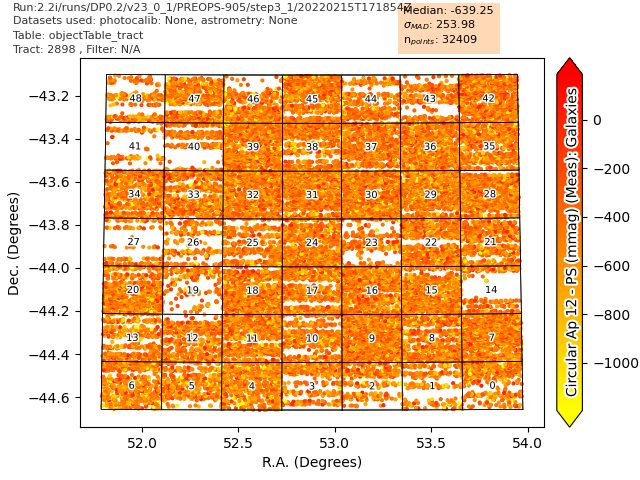
\includegraphics[width=0.7\textwidth]{coadd_bug.png}
\caption{The regions of the coadd that lack any Objects were caused by an unexpected failure mode in
    accessing the input images, which was possible on cloud infrastructure but not seen on POSIX
    files. \label{fig:coadd}}
\end{figure}

The data previews are also a chance to learn from the issues that we didn’t catch during V\&V; most
notably were two cases where invalid flux calibrations were being applied to certain measurement
algorithms, resulting in NaNs in the output. This case shows the value of having a wide breadth of
testing coverage. For future releases we will ensure that we have some form of testing for every
column in every user-facing data product. Even if the tests are relatively simple, they may identify
significant issues.

As one further example of potential issues encountered during production, a few days after the start
of single frame processing the pipelines began to show hundreds of failures with the error message
\texttt{Exception ValueError: No reference objects supplied}. This was not seen in the pilot run, so
production was paused while we investigated. By plotting the locations of these failures on the sky,
we determined that these sensors fell outside the footprint of the stellar input catalog, and hence
there were no stars available for calibrating these images. These were thus “unprocessable” and no
corrective action was required, but it illustrated the value of realtime error collection and
monitoring during production.


\section{Science Platform, user front end for DP0.2 } \label{sec:frontend}

DP0.1 upgrade image services any new issues  but mainly deployment and control, issue handling

\subsection{Qserv}\label{sec:qserv}

Qserv is a horizontally scalable parallel SQL database system, developed by the Rubin Observatory specifically
to support the LSST production catalog use case.  Qserv is further described in \citeds{LDM-135}.

The DP0.2 simulated survey covers about 1/60th of the anticipated on-sky area of the full survey (roughly
300/18,000 sq. degrees), at about half the anticipated observational depth of the full survey.  The generated
catalogs contain \textasciitilde{}136 billion rows in total.  On disk, including necessary indexes, this
amounts to \textasciitilde{}30 TiB of database storage.  A Qserv cluster with one head node and five worker
nodes was comissioned in the IDF cloud computing environment to host and serve this data.

\subsubsection{Enhancements delivered during DP0.2}

\begin{itemize}

\item
  \textbf{Ingest systems:} At these scales, a trouble-free database ingest from DRP pipeline outputs to a
  complete online database takes several days.  All catalog data must be format converted from the parquet
  outputs as delivered by DRP to CSV files needed for efficient load at the Qserv worker nodes.  Data after
  conversion must be sharded, distributed, loaded at worker nodes, and appropriate indices compiled.  A
  significant fraction of the Qserv codebase is concerned only with the management, tracking, and automation
  of these ingest activities.

  Enhancement of these Qserv subsystems continued during the course of the DP0.2 exercise, and improvements
  were deployed continuously into production.  These improvments were aimed at streamlining the ongoing ingest
  campaigns, and included such features as provision of fully asynchronous task APIs to upstream ingest
  tooling, refinements to the ingest state machine for improved observability of ongoing ingest activities,
  and finer-grained control over publication/retraction/replacement life-cycle of individual tables.

\item
  \textbf{Diagnostic monitoring:} Qserv provides its own in-built administration dashboard, which has proved
  to be an indispensible tool for monitoring and troublshooting operating instances.  This subsystem also saw
  lots of improvement during the course of DP0.2, including instrumentation of many additional aspects of
  Qserv related to ingest and query processing activities, an enhanced query monitor / query history, and
  overall performance improvments to the administration dashboard itself.

\item
  \textbf{Optimized point-in-polygon spherical geometric queries:} Rather late in timeline for DP0.2 a
  decision was taken to host IVOA ObsCore observational metadata within Qserv, since doing so would enable a
  much richer interaction model with image data and image services being offered for the first time in DP0.2.
  This interaction model required support for point-in-polygon spherical geometry queries, and needed spatial
  indexing features beyond the previously established scope of Qserv for DP0.2 in order to perform acceptably.
  A workable strategy for efficiently processing these sorts of queries based on integration of several bits
  of existing functionality was developed and successfully delivered into production.

\item
  \textbf{Photometry UDFs:} Some photometry-related UDFs were developed and contributed upstream to the SciSQL
  project (https://github.com/smonkewitz/scisql), along with general modernization and infrastructural
  improvements of SciSQL.  These UDFs can simplify construction of queries against the LSST data model, which
  to date is committed to provision of linear flux measurements rather than logarithmic magnitudes
  (\citeds{Document-27758}).

\end{itemize}

\subsubsection{Some lessons learned}

DP0.2 proved to be a very valuable exercise in shaking down Qserv and surrounding tooling and operating
processes.  Some take-aways related providing catalog database service for DP0.2:

\begin{itemize}

\item
  \textbf{Timely schema metadata is hard to get.}  Rubin's middleware has an extremely flexible data
  model.  While this provides a lot of agility in pipeline development, when it comes to provision of
  catalog services at some point before database ingestion a concrete schema commitment must be made.

  While Rubin does have an accepted format for such schema descriptions and a sufficient source control and
  deployment practice around this, the schema descriptions themselves run to the many thousands of lines and
  nobody chomps at the bit to make sure these are maintained, current, complete, and error free.  Otherwise
  ready-to-go catalogs have on more than one occasion been held up in release by the need for last-minute
  revisions to the schema descriptions.

  Remediation: much has been done already to drive schema consumers toward a single source of truth and to
  streamline the deployment and update of schemas, once updates are committed to source control.  Since
  schema description deliverables have consistently been seen to lag, it remains for management to
  appropriately pre-load the demand for these.

\item
  \textbf{Data curation -- try (even) harder.}  Often times, catalog data curation issues are not easily
  detected until the "end of the line", when a completed data release is presented for database ingestion.
  Representation issues, key constraints, and referential integrity issues may not be apparent until a full
  set of tables is available.  Some curation issues may not even be detected until \emph{after} database
  ingestion, when the catalogs can first conveniently be queried in the large.

  For DP0.2, there was a plan to mitigate turbulence at the end of the line by obtainin and ingesting a
  representationally complete subset of catalog products early in the release cycle.  In practice, this had
  only limited success.  Inevitable delays on all fronts compressed the time between availability of the
  subset products and the full release products.  Additionally, sequencing of DRP activity meant while some
  subset tables were available usefully early in the release cycle, others were not available until much
  later, closer to the full release.  Predictably, curation issues \emph{did} exist that thus were not
  identified until fairly late in the release cycle, and release of several tables in the data products was
  delayed while these tables were re-processed upstream and then re-ingested into the database.

  Remediation: work with DRP to see if a more complete set of tables can feasibly be obtained earlier in the
  release cycle. Schedule subset production and ingest even more conservatively.

\item
  \textbf{Watch out for automated test lacunae.}  Qserv contains some distributed reference match machinery to
  facilitate performant joins between catalogs.  It turns out that DP0.2 includes a truth table and associated
  match table which depend upon this functionality.  Though this feature is not otherwise commonly in use, the
  Qserv development team maintained a high level of confidence that it was ready to go, because it had known
  coverage in the automated integration test suites, and "if it was broken, we'd know about it."

  As it turned out, the relevant integration tests had been commented out of the test suite sometime in the
  previous year as a temporary measure while working through some containerization/deployment issues, test
  coverage had never been subsequently restored, and the uncovered feature, when put into use, was found to
  have some minor issues.

  Remediation: a thorough survey of the test suites was conducted, and commented/disabled tests were updated
  as necessary and returned to active service.

\end{itemize}



\section{Community engagement} \label{sec:cet}

As for DP0.1 CET gathers documentation and tuturial informaiton on \url{https://dp0-2.lsst.io/}.



\appendix
% Include all the relevant bib files.
% https://lsst-texmf.lsst.io/lsstdoc.html#bibliographies
\section{References} \label{sec:bib}
\renewcommand{\refname}{} % Suppress default Bibliography section
\bibliography{local,lsst,lsst-dm,refs_ads,refs,books}

% Make sure lsst-texmf/bin/generateAcronyms.py is in your path
\section{Acronyms} \label{sec:acronyms}
\addtocounter{table}{-1}
\begin{longtable}{p{0.145\textwidth}p{0.8\textwidth}}\hline
\textbf{Acronym} & \textbf{Description}  \\\hline

CAM & CAMera \\\hline
DC2 & Data Challenge 2 (DESC) \\\hline
DESC & Dark Energy Science Collaboration \\\hline
DM & Data Management \\\hline
DMCCB & DM Change Control Board \\\hline
DMTR & DM Test Report \\\hline
DP0 & Data Preview 0 \\\hline
DPLT & DP Leadership Team \\\hline
DRP & Data Release Production \\\hline
FrDF & French Data Facility \\\hline
LSST & Legacy Survey of Space and Time (formerly Large Synoptic Survey Telescope) \\\hline
NCSA & National Center for Supercomputing Applications \\\hline
OPS & Operations \\\hline
RTN & Rubin Technical Note \\\hline
T/CAM & Technical/Control (or Cost) Account Manager \\\hline
UKDF & United Kingdom Data Facility \\\hline
USDF & United States Data Facility \\\hline
\end{longtable}

% If you want glossary uncomment below -- comment out the two lines above
%\printglossaries





\end{document}
